\documentclass[a4paper,11pt]{article}

\usepackage[margin=3cm]{geometry}
 
\usepackage{graphicx}
\usepackage{subcaption}
\usepackage[colorlinks,allcolors=violet]{hyperref}
\usepackage{url}

% https://tex.stackexchange.com/questions/94032/fancy-tables-in-latex
\usepackage[table]{xcolor}
\usepackage{booktabs}

\usepackage[utf8]{inputenc}
\usepackage{pdfpages}

% https://tex.stackexchange.com/questions/664/why-should-i-use-usepackaget1fontenc
\usepackage[T1]{fontenc}
\usepackage{lmodern} 

\usepackage{float}

% https://www.overleaf.com/learn/latex/Aligning_equations_with_amsmath
\usepackage{amsmath}

% Packages to use TikZ
\usepackage{tikz}
\usepackage{tikzscale}
\newlength\figureheight % used to control the size of TikZ figures
\newlength\figurewidth
\usepackage{pgfplots}
\usetikzlibrary{positioning} % for the relative positions of nodes in TikZ figures

\newcommand{\note}[1]{{\colorbox{yellow!40!white}{#1}}}
\newcommand{\exampletext}[1]{{\color{blue!60!black}#1}}

% Package to add code
\usepackage{listings}

% Parameters for highlighting javascript code, you are certainly allowed to change this.
\definecolor{lightgray}{rgb}{.9,.9,.9}
\definecolor{darkgray}{rgb}{.4,.4,.4}
\definecolor{purple}{rgb}{0.65, 0.12, 0.82}

% See https://github.com/ghammock/LaTeX_Listings_JavaScript_ES6

\lstdefinelanguage{JavaScript}{
  morekeywords=[1]{break, continue, delete, else, for, function, if, in,
    new, return, this, typeof, var, void, while, with},
  % Literals, primitive types, and reference types.
  morekeywords=[2]{false, null, true, boolean, number, undefined,
    Array, Boolean, Date, Math, Number, String, Object},
  % Built-ins.
  morekeywords=[3]{eval, parseInt, parseFloat, escape, unescape},
  sensitive,
  morecomment=[s]{/*}{*/},
  morecomment=[l]//,
  morecomment=[s]{/**}{*/}, % JavaDoc style comments
  morestring=[b]',
  morestring=[b]"
}[keywords, comments, strings]

\lstalias[]{ES6}[ECMAScript2015]{JavaScript}

\lstdefinelanguage[ECMAScript2015]{JavaScript}[]{JavaScript}{
  morekeywords=[1]{await, async, case, catch, class, const, default, do,
    enum, export, extends, finally, from, implements, import, instanceof,
    let, static, super, switch, throw, try, string, interface}, % string and interface added
  morekeywords=[2]{Map, Set},
  morestring=[b]` % Interpolation strings.
}

\lstset{
	language=ES6,
	extendedchars=true,
	basicstyle=\footnotesize\ttfamily,
	showstringspaces=false,
	showspaces=false,
	numbers=left,
	numberstyle=\footnotesize,
	numbersep=9pt,
	tabsize=2,
	breaklines=true,
	showtabs=false,
	captionpos=b,
	keywordstyle=\color{blue}\bfseries,
	identifierstyle=\color{black},
	commentstyle=\color{purple}\ttfamily,
	stringstyle=\color{red}\ttfamily,
}


\begin{document}

\noindent
\colorbox[HTML]{52BDEC}{\bfseries\parbox{\textwidth}{\centering\large
  --- P\&O CW 2023--2024: Story Book Report ---
}}
\\[-1mm]
\colorbox[HTML]{00407A}{\bfseries\color{white}\parbox{\textwidth}{
  Department of Computer Science -- KU Leuven
  \hfill
  \today
}}
\\

\smallskip

\noindent
%\mbox{}\hfill
\begin{tabular}{*2l}
% Provide the git tag name and a clickable link in the \href command:
\multicolumn{2}{l}{\large\textbf{Team <00>: \href{https://gitlab.kuleuven.be/p-en-o-cw/2022-2023/story-book/ngram}{<git-tag-link>}}} \\
\midrule
<first name last name>   & 0h \\ % fill in the estimated time spend on P&O CW per team member for the full semester up till now, including the lab sessions
<first name last name>   & 0h \\
...\\
\bottomrule
\hline
\end{tabular}

\noindent\note{\parbox{\textwidth}{{Fill in the estimated time spent on P\&O CW per team member for the full semester up till now, including the lab sessions.}}}

\bigskip

\noindent
{\color[HTML]{52BDEC} \rule{\linewidth}{1mm} }

\vspace{-6mm}
\section*{Focus points}
This part will be filled in by the teaching team.
\bigskip

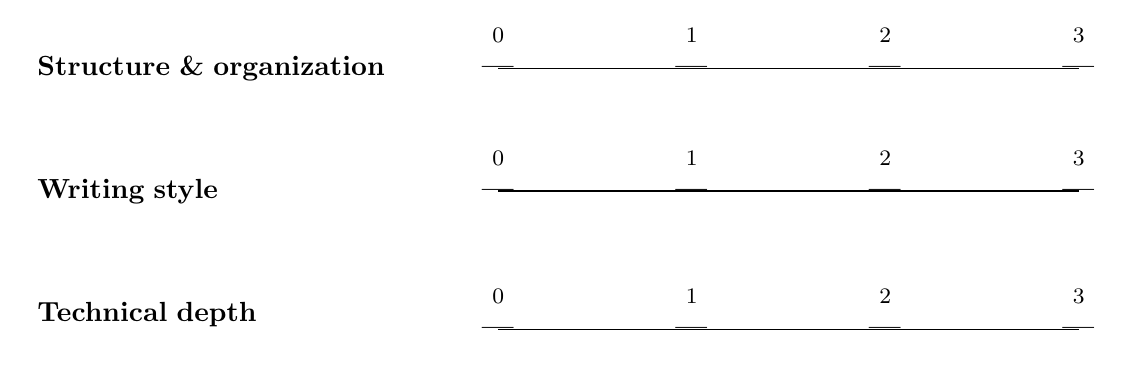
\begin{tikzpicture}[
  roundnode/.style={circle, draw=white, fill=white, inner sep=0pt, minimum size = 1mm},
  squarednode/.style={rectangle, draw=white, fill=white, text width=5cm},
  scorenode/.style={rectangle, draw=white,inner sep =0pt, outer sep=0}
  ]
  % Focus points
  \node[squarednode]  (maintopic1)                             {\textbf{Structure \& organization}};
  \node[squarednode]  (maintopic2)    [below=of maintopic1]    {\textbf{Writing style}};
  \node[squarednode]  (maintopic3)    [below=of maintopic2]    {\textbf{Technical depth}};
  
  % Grading grid nodes
  \node[roundnode]    (score11)       [right=0.5cm of maintopic1]    {\textbf{|}};
  \node[roundnode]    (score12)       [right= 2cm of score11]       {\textbf{|}};
  \node[roundnode]    (score13)       [right= 2cm of score12]       {\textbf{|}};
  \node[roundnode]    (score14)       [right= 2cm of score13]       {\textbf{|}};
  \node[roundnode]    (score21)       [right=of maintopic2, below=1.1cm of score11]    {\textbf{|}};
  \node[roundnode]    (score22)       [below=1.1cm of score12]       {\textbf{|}};
  \node[roundnode]    (score23)       [below=1.1cm of score13]       {\textbf{|}};
  \node[roundnode]    (score24)       [below=1.1cm of score14]       {\textbf{|}};
  \node[roundnode]    (score31)       [right=of maintopic3, below=1.3cm of score21]    {\textbf{|}};
  \node[roundnode]    (score32)       [below=1.3cm of score22]       {\textbf{|}};
  \node[roundnode]    (score33)       [below=1.3cm of score23]       {\textbf{|}};
  \node[roundnode]    (score34)       [below=1.3cm of score24]       {\textbf{|}};
  
  % Grading grid lines
  \draw[-] (score11.center) -- (score14.center);
  \draw[-] (score21.center) -- (score24.center);
  \draw[-] (score31.center) -- (score34.center);
  
  % Grading labels
  \node[scorenode]    (label1)        [above=1mm of score11]       {\footnotesize	 0};
  \node[scorenode]    (label2)        [above=1mm of score12]       {\footnotesize	 1};
  \node[scorenode]    (label3)        [above=1mm of score13]       {\footnotesize	 2};
  \node[scorenode]    (label4)        [above=1mm of score14]       {\footnotesize	 3};
  
  \node[scorenode]    (label6)        [above=1mm of score21]       {\footnotesize	 0};
  \node[scorenode]    (label7)        [above=1mm of score22]       {\footnotesize	 1};
  \node[scorenode]    (label8)        [above=1mm of score23]       {\footnotesize	 2};
  \node[scorenode]    (label9)        [above=1mm of score24]       {\footnotesize	 3};
  
  \node[scorenode]    (label11)       [above=1mm of score31]       {\footnotesize	 0};
  \node[scorenode]    (label12)       [above=1mm of score32]       {\footnotesize	 1};
  \node[scorenode]    (label13)       [above=1mm of score33]       {\footnotesize	 2};
  \node[scorenode]    (label14)       [above=1mm of score34]       {\footnotesize	 3};
  
  \end{tikzpicture}

  \noindent
  {\color[HTML]{52BDEC} \rule{\linewidth}{1mm} }

\exampletext{
  \paragraph{Practical guidelines}
  \begin{itemize}
      \item This report should be no longer than 4 pages.
      \item Add your team number, names and time spent at the top of the report. Remove the angular brackets in the heading.
      \item Mark the author of a section or a paragraph in the margin using \texttt{marginpar}. You can abbreviate the names.
      \item Delete all the blue guidelines and the section ``\LaTeX~Tips \& Tricks" from your final report before submitting.
  \end{itemize}  
\paragraph{Content guidelines}
\begin{itemize}
  \item The main deliverable of the Story Book assignment is the Reverse Dictionary Search feature: Given a description of a word, inputted via the command line, present a list of words that match this description.
  \item In this report, we want you to document how your team tackled this problem. Think of it as a miniature of the report you will be submitting at the end of the semester. Pay attention to its structure. Use academic language and writing style.
  \item Discuss and evaluate your solution on a technical level. What did you implement? How did you implement it, and why? How did you test it? How good does the implementation work? You should of course report on the results as well.
  \item Also discuss the learning process. We want to know how you approached the task, e.g., how tasks were divided, which difficulties were encountered, ... You can also discuss technical difficulties encountered with Git, Node and/or Typescript.
  \item Write the report for an audience with similar background knowledge as yourself. Avoid over-explaining basic concepts, but remember that a report should state the problem at hand, such that it is self-contained.
\end{itemize}
}

\reversemarginpar
\section{\LaTeX~Tips \& Tricks}\label{sec:Feature}
\marginpar{KB,DD} 
\note{Mention authors in the margin.}\\
There is a lot of things you can do with \LaTeX. We give examples of how to include figures, tables, code snippets, \dots, as well as how to reference them and use citations.

\subsection{Tables and referencing}\label{ssec:tables}
\marginpar{KB} 

Using the \texttt{booktabs} package, you can create professional looking tables. An example is given in Table~\ref{tab:example}, which we were just able to reference automatically using \verb|\ref{...}|. You can reference many things, as long as you give them a label using \verb|\label{...}|. Even though numbering may change, the reference will always be correct, like the fact that this is Subsection~\ref{ssec:tables}.

Table cells are separated with \verb|&| and rows are ended with \verb|\\|. The construction looks like this in general:
\begin{verbatim}
  \begin{table}[h]
    \centering % comment: center the table
    \begin{tabular}{...}
      ...
    \end{tabular}
    \caption{...}\label{...}
  \end{table}
\end{verbatim}
After \verb|\begin{tabular}|, you specify the number of columns and their alignment, e.g.\ \verb|{l c c c c}|.

\begin{table}[h]
  \centering
\begin{tabular}{l c c c c}
  \toprule
& \multicolumn{4}{c}{explanation} \\
\cmidrule(l){2-5}
Topic & col 1 & col 2 & col 3 & col 4 \\
\midrule % In-table horizontal line
hor.\ lines & \verb|\toprule| & \verb|\midrule| & \verb|\bottomrule| & \verb|\cmidrule(l){2-6}| \\
multicolumn & `explanation' & is done with & \verb|&\multicolumn| & \verb|{4}{c}{...}| \\
\midrule
\midrule
positioning & \texttt{[h]}(here) & \texttt{[t]}(top) & \texttt{[b]}(bottom) & \texttt{[p]}(separate page) \\
\bottomrule
\end{tabular}
\caption{This is inside a \texttt{\textbackslash caption\{\dots\}} construction and following it by \texttt{\textbackslash label\{\dots\}} allows you to reference this table.}
\label{tab:example}
\end{table}

\subsection{Figures and citations}
\marginpar{KB,DD} 

Figures can be included using the \texttt{graphicx} package. An example is given in Figure~\ref{fig:gitlab-icon}. The construction looks like this in general:
\begin{verbatim}
  \begin{figure}[h]
    \centering
    \includegraphics[width=<ratio>\textwidth]{<file>}
    \caption{...}\label{...}
  \end{figure}
\end{verbatim}
You can also create figures in \LaTeX~using TikZ~\cite{website:TikZ}. An example is given in Figure~\ref{fig:node}. In this case, you use \verb|\input{...}| instead of \verb|\includegraphics{...}| to include the TikZ figure defined in a separate file.

\begin{figure}[h]
  \centering
  
\includegraphics[width=0.3\textwidth]{figures/gitlab-icon.png}
  \caption{Always remember to explain what is in the figure. This is a picture of the Gitlab icon.}
  \label{fig:gitlab-icon}
\end{figure}

\begin{figure}[!ht]
	\centering
	\setlength\figureheight{3cm}
	\setlength\figurewidth{5cm}
	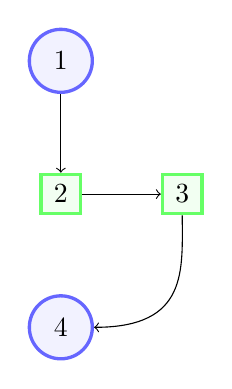
\begin{tikzpicture}[
roundnode/.style={circle, draw=blue!60, fill=blue!5, very thick, minimum size=8mm},
squarednode/.style={rectangle, draw=green!60, fill=green!5, very thick, minimum size=5mm},
]
%Nodes
\node[squarednode]      (maintopic)                              {2};
\node[roundnode]        (uppercircle)       [above=of maintopic] {1};
\node[squarednode]      (rightsquare)       [right=of maintopic] {3};
\node[roundnode]        (lowercircle)       [below=of maintopic] {4};

%Lines
\draw[->] (uppercircle.south) -- (maintopic.north);
\draw[->] (maintopic.east) -- (rightsquare.west);
\draw[->] (rightsquare.south) .. controls +(down:7mm) and +(right:12mm) .. (lowercircle.east);





\end{tikzpicture}

	\caption{TikZ example.}
	\label{fig:node}
\end{figure}

Notice how we added an automatic citation to the Tikz website in the previous paragraph? This is done using the \verb|\cite{...}| command. The references are managed in a separate file, \texttt{references.bib}, and are included at the end of the document using the \verb|\bibliography{...}| command. If you add the proper information in the \texttt{.bib} file, the citation will be automatically formatted. The style of the bibliography can be changed by changing the argument of the \verb|\bibliographystyle{...}| command. Remember to put the citations in the right place in the text though, e.g.\ if I cite the \texttt{pgfplots} package~\cite{website:pgfplots}, I put the citation right after, and not after the whole sentence.

\subsection{Equations and code snippets}
\marginpar{DD} 

There are a lot of ways to include equations in \LaTeX. You can use the \verb|equation| environment to include a single equation, or the \verb|align| environment to include multiple equations. An example is given in Equation~\ref{eq:example}. Alternatively, you can use the \verb|$$...$$| or \verb|\[...\]| constructions. To insert an equation like $E=mc^2$ or \(F=ma\) directly in the text, you can use \verb|$...$| or \verb|\( ...\)|.

\begin{equation}
  \label{eq:example}
  \begin{split}
    \nabla \cdot \vec{E} &= \frac{\rho}{\varepsilon_0} \\
    \nabla \times \vec{E} &= -\frac{\partial \vec{B}}{\partial t}
  \end{split}
\end{equation}

To reference an equation like `(\texttt{<number>})', you can use \verb|\eqref{...}|: In \eqref{eq:example} we actually used the \verb|split| environment from the \texttt{amsmath} package to align the equations. If we had used the \verb|align| environment, we would have gotten a number for each line. We can also remove the numbering by adding an asterisk to the environment name, e.g.
\begin{verbatim}
  \begin{equation*}
    ...
  \end{equation*}
\end{verbatim}
would not have numbered the equation. In general, you only want to number the equations you are going to reference later.

Throughout the examples, we have listed \LaTeX~code snippets using the \verb|verbatim| environment. To include code snippets from a programming language, you can use the \texttt{listings} package. An example of how to do this is
\begin{verbatim}
  \begin{lstlisting}[ language=ES6, 
                      caption={Example of a code snippet.}, 
                      label={lst:example}]
    const example = (a, b) => {
      return a + b;
    }
  \end{lstlisting}
\end{verbatim}
which results in Listing~\ref{lst:example}. The \texttt{language} parameter specifies the language of the code, which is used to highlight the code properly. The \texttt{caption} and \texttt{label} parameters are used to give the code snippet a caption and a label, respectively. We have configured the \texttt{ES6} language option in the preamble to highlight JavaScript code.

\begin{lstlisting}[ language=ES6, 
                    caption={Example of a code snippet.}, 
                    label={lst:example}]
const example = (a, b) => {
return a + b;
}
\end{lstlisting}


%%%%%%%%%%%%%%%%%%%%%%%%%%%%%%%%%%%%%%
\newpage
\bibliographystyle{plain}
\bibliography{references}

%%%%%%%%%%%%%%%%%%%%%%%%%%%%%%%%%%%%%%

\end{document}
